之前已经讨论了 MBPT 的多种变体——单参考态计算闭壳核,多参考态,以及 $\hat{Q}$-box 导出有效相互作用。众所周知,关联对于描述多体系统至关重要,除了包含所有关联的 FCI 之外,多体方法应尽可能包含更多的关联,才能得到多体系统的较好结果。除了 MBPT 之外,IMSRG 以及 CC 是两种常用的非微扰的多体方法,那这三种方法各自将关联包含到了什么层次呢?

关联是个非常神奇的东西,以闭壳核为例,使用只包含到两体力的哈密顿量(以下讨论也都不包含三体力),$0p0h$ 的组态最多只会与 $2p2h$ 的组态有相互作用,但 $2p2h$ 还可以继续与 $4p4h$ 有相互作用,这样一系列组态就都有复杂的嵌套的关联。全组态相互作用方法在组态表象下写出组态空间哈密顿量并对角化,可以将所有的关联都包含进去。但因为组态空间的维数太大,这种做法对于稍重一点的核就不可行,一定需要截断组态基。

\section{MBPT}
MBPT 是组态空间中的方法,在这里讨论单参考态 MBPT 计算闭壳核,以及 $\hat{Q}$-box 得到价空间有效相互作用这两种形式,均在组态空间中考虑问题。闭壳核的组态空间基矢形如 $npnh$,单参考态 MBPT 做的事情其实是通过将能量与波函数分为各阶微扰,以此对组态空间哈密顿量的本征值方程进行变形,避免了一次性处理所有的组态基,纳入考虑的组态基随着微扰阶数的增加逐渐增多,当考虑到 $n$ 阶微扰时,微扰能量的中间态最多为 $2(n-1)p2(n-1)h$,微扰波函数则最多能包含 $2np2nh$。所以其实可以将 MBPT 的阶数截断(部分)认为是对组态空间基矢进行截断。\underline{如果能够算到无穷阶微扰且收敛,应该等价于组态相互作用的直接对角化},因为 MBPT 是直接由组态相互作用的本征值方程推导出来的,除了微扰之外没有做其他假设与截断。(这个判断是我个人的观点,没有从别处看到过类似的表述,但我有自信这是正确的,当然实际上不可能算到无穷阶,所以是一句正确的废话)

微扰阶数截断只能 \underline{部分} 认为是对基矢的截断,是因为算到 $n$ 阶微扰时并没有完整包含低于 $2(n-1)p2(n-1)h$ 的所有关联,并不能像截断的组态相互作用那样,截断到 $npnh$ 就能包含低于 $npnh$ 的所有关联。这是由 MBPT 的微扰特性决定的。为了方便说明,考虑一个闭壳 MBPT 的高阶图 \ref{fig:csmbpt-5th}。在二阶微扰中就有类似的图,中间态是 $2p2h$,但可以在二阶图中间添加无数条相互作用线,$2p2h$ 中间态会出现很多次,此时阶数就会变得很高,比如五阶的图 \ref{fig:csmbpt-5th}。但中间态仍然只有 $2p2h$,这说明 $0p0h$ 与 $2p2h$ 的关联会分散到各阶中,不算到无穷阶的话,就连 $0p0h$ 与 $2p2h$ 的耦合都退不干净。

\begin{figure}[!htbp]
    \centering
    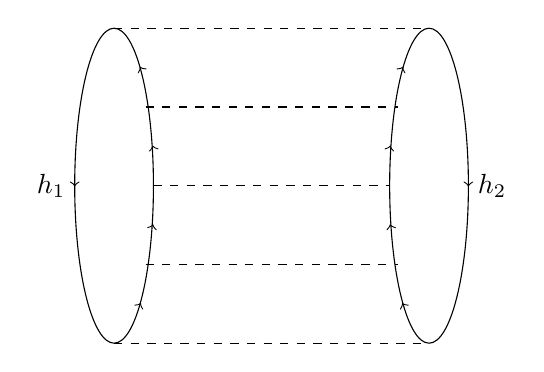
\begin{tikzpicture}
        \draw[-] (0,2) ellipse [x radius=0.5, y radius=2];
        \draw[-] (4,2) ellipse [x radius=0.5, y radius=2];
        \draw[dashed] (0,0)--(4,0);
        \draw[dashed] (0.4,1)--(3.6,1);
        \draw[dashed] (0.5,2)--(3.5,2);
        \draw[dashed] (0.4,3)--(3.6,3);
        \draw[dashed] (0,4)--(4,4);
        \draw[->] (-0.5,2.01)--(-0.5,1.99);
        \draw[->] (4.5,2.01)--(4.5,1.99);
        \draw[->] (0.33,0.49)--(0.34,0.51);
        \draw[->] (0.34,3.49)--(0.33,3.51);
        \draw[->] (3.67,0.49)--(3.66,0.51);
        \draw[->] (3.66,3.49)--(3.67,3.51);
        \draw[->] (0.49,1.49)--(0.495,1.51);
        \draw[->] (0.495,2.49)--(0.49,2.51);
        \draw[->] (3.51,1.49)--(3.505,1.51);
        \draw[->] (3.505,2.49)--(3.51,2.51);
        \node at (-0.8,2) {$h_1$};
        \node at (4.8,2) {$h_2$};
    \end{tikzpicture}
    \caption{\label{fig:csmbpt-5th}闭壳 MBPT 的五阶图,所有中间态都是 $2p2h$。}
\end{figure}

\section{$\hat{Q}$-box}
MBPT 得到有效相互作用与之前讨论的 MBPT 不同,没有参考态的说法。有效相互作用公式推导的核心是相似变换后的哈密顿量 $\mathcal{H}$ 如果满足 $Q\mathcal{H}P=0$,就能保证 $P\mathcal{H}P$ 的本征值与最初的 $H$ 相同。从 $Q\mathcal{H}P=0$ 出发,以 Lee-Suzuki 相似变换进行化简,也会出现 $QHQ$ 这样的项。从数学角度来看,相似变换后使 $Q\mathcal{H}P=0$,只对 $QHP$ 进行操作是不可能完成的,一定要同时操作 $QHQ$。从物理角度来看,退耦合 $P$ 与 $Q$ 空间的态,会不可避免地涉及到 $Q$ 空间内部的耦合,这也是之前提及的组态间的关联嵌套的体现。

除了微扰导致关联考虑不全的问题之外,$\hat{Q}$-box 有效相互作用还有一个问题,就是之前提到的 valence cluster expansion(VCE)。因为 MBPT 实际操作的都是组态相互作用的矩阵,但对于核芯上填 $A_v$ 个粒子的体系,应该存在一条,两条乃至 $A_v$ 条外腿的图。这些图全部纳入计算的难度太大了,因此 VCE 的思想是计算核芯上填充一个与两个核子的情况,此时只用计算一条与两条外腿的图。对一价核子与二价核子体系退耦合,得到适用于这些核的有效相互作用后,认为这个有效相互作用适用于整个壳,这就是 $\hat{Q}$-box 这种多体方法的截断。

随着核子数的增多,这么做从直觉上来看就不合适。少价核子体系的有效相互作用与更多核子体系的不应该相同,看上去很显然,但还不够有说服力。回顾具体求解过程,先对一核子体系求解 $\hat{S}$-box,得到有效相互作用的单体部分,再对二价核子体系求解 $\hat{Q}$-box,此时得到的 $P\mathcal{H}P$ 是二价核子体系的组态空间哈密顿量,并不是 Fock 空间的有效相互作用,需要从中减去单体部分才能得到有效相互作用的两体部分。如果继续考虑三价核子体系,需要减去单体与两体部分得到有效相互作用的三体部分。可以发现 $A_v$ 价核子体系的单体、两体直至 $A_v-1$ 体就是通过更少价核子体系获得的,求解 $A_v$ 价核子体系只是为了更新 $A_v$ 体部分。也就是说,在 $\hat{Q}$-box 的理论框架下,壳中其他原子核的单体和两体部分就等于只包含到两体图的有效相互作用。问题在于更多体部分直接缺失掉了。如果想包含这部分的影响,最直接的方式当然是使用能直接考虑三体部分的壳模型,退而求其次的方法是将这部分等效考虑进一体与二体,比如算二阶三体图 \cite{2019ma,2020coraggio-2vbetabeta,2020coraggio-ca,2022coraggio}。

VCE 导致关联缺失,所以结果算不准是显然的。也可以回归到有效相互作用理论的出发点看看 VCE 带来了什么。VCE 会导致退耦不干净,进而使模型空间的组态相互作用对角化与 FCI 产生偏差。这是因为对于大于两价核子的原子核,使用包含到两体图的有效相互作用,等价于这个相似变换没有清空 $Q\mathcal{H}P$,因为能清空 $Q\mathcal{H}P$ 的相似变换必然使 $P\mathcal{H}P$ 出现三体项,如果没有,耦合就没有完全退去。此外,阶数的截断也会导致 $Q\mathcal{H}P$ 不能完全清空。

\section{VS-IMSRG}
\subsection{退耦方式}
相比 MBPT,VS-IMSRG 直接操作 Fock 空间的哈密顿量。Fock 空间是所有粒子数的 Hilbert 空间的张量积。VS-IMSRG 的核心思想是,通过连续的相似变换将 Fock 空间的哈密顿量非对角元压低至 0,非对角元可以任意选取,这正是 IMSRG 直接推广到 VS-IMSRG 的方便之处。VS-IMSRG 选取的非对角元正是指标中涉及到模型空间外的态的矩阵元。这样做的好处是,用相似变换后的 Fock 空间哈密顿量 $H(s\to\infty)$ 写出组态空间哈密顿量 $\mathcal{H}$ 时,$Q\mathcal{H}P$ 块为 0,因为 $H(s\to\infty)$ 的矩阵元中涉及 $P$ 与 $Q$ 轨道耦合的项全都被演化为 0 了,自然就能保证 $P\mathcal{H}P$ 对角化与 FCI 得到一样的结果。

非对角元的选取不能太任意,出于计算考虑,非对角元选取过于广泛的话会导致对易中诱导出大量的三体算符,IMSRG(2) 截断失效 \cite{2017hergert}。这里先讨论退耦是怎么实现的。$Q\mathcal{H}P$ 的矩阵元可以用图 \ref{fig:imsrg-QHP} 的两体组态空间的矩阵元代表,更多粒子的组态空间相当于在此基础上添加旁观粒子,而单粒子组态空间则是去掉一个旁观粒子,都不影响这五种矩阵元的表达式。只需要将组成这五个组态空间的矩阵元的 Fock 空间非对角元演化为 0,就能保证 $Q\mathcal{H}P=0$。这里直接给出结果:

\begin{equation}
    H^{\mathrm{od}}=\{f_{ph},f_{pp^{\prime}},f_{hh^{\prime}},\Gamma_{pp^{\prime}hh^{\prime}},\Gamma_{pp^{\prime}vh},\Gamma_{pqvv^{\prime}}\}+\mathrm{H.c.}.\label{eqs:imsrg-Hod1}
\end{equation}

\begin{figure}[htbp]
  \centering
  \includegraphics[width=0.9\textwidth]{figure/imsrg-QHP.png}
  \caption{VS-IMSRG 退耦合的 $Q\mathcal{H}P$ 矩阵元,图取自 \cite{2017hergert}。}
  \label{fig:imsrg-QHP}
\end{figure}

注意这些需要压低的非对角元全是 normal order 后的矩阵元。
接下来用没有 normal order 的组态相互作用的公式推导这五类矩阵元,来得到需要压低的 Fock 空间非对角元。从下面的推导中可以看出,用没有 normal order 的哈密顿量进行推导,五种矩阵元有一系列的求和,形式比较复杂,如果把所有出现在求和中的非对角元全部压低为 0 会很麻烦。不过这些求和都能用 normal order 的哈密顿量简单地表示,所以直接压低 normal order 的非对角元更加容易。这也是 IMSRG 选择在 normal order 的公式形式下工作的另一个原因,首要原因自然是为了包含三体力。

直接使用最简洁的组态相互作用公式 \ref{eqs:ci-0},\ref{eqs:ci-1} 与 \ref{eqs:ci-2}。
在接下来的推导中,考虑价核子与核芯的存在,将组态写为 $|D\rangle=\prod_{i=1}^{m}a_{v_i}^\dagger\prod_{j=1}^{n}a_{c_j}^\dagger|0\rangle$,有 $m$ 个价核子,核芯有 $n$ 个核子,并不局限于两价核子空间。

第一类矩阵元是一个价核子由价空间轨道 $v_a$ 到价空间之外的 $q_b$,其他价核子都旁观,也就是 
\begin{equation}
    |D_f\rangle = \prod_{i\ne a} a_{v_i}^\dagger a_{q_b}^\dagger\prod_{j=1}^{n}a_{c_j}^\dagger|0\rangle,
\end{equation}
因此 
\begin{equation}
    \langle D_f|H|D_i\rangle_\mathrm{I} = (-1)^{\mathrm{permute}(v_a,q_b)}\left(h_{q_bv_a}+\sum_{k=1}^nV_{q_bc_kv_ac_k}+\sum_{l\ne a}V_{q_bv_lv_av_l}\right),
\end{equation}
$c_k$ 是对 hole 的求和,因此 
\begin{equation}
    h_{q_bv_a}+\sum_{k=1}^nV_{q_bc_kv_ac_k}=f_{q_bv_a},
\end{equation}
对核芯进行 normal order 时,$n_k=\theta(\epsilon_\mathrm{F}-\epsilon_k)$,也就是占据数只能为 0 或 1,前两项之和就变成了 normal order 后的单体项,这一项形如 $f_{qv}$,但对应非对角元的 $f_{pp'}$。而第三项形如 $\Gamma_{vqv'v''}$,但非对角元的选取是 $\Gamma_{pqvv'}$,这么定义是为了同时使第二类矩阵元也为 0。因为第三项是两体相互作用,应该出现在第二类矩阵元的图中,这是因为第一类矩阵元是用差 1 个轨道的组态相互作用公式计算的,也会包含差 2 个轨道的退化情况。

第二类矩阵元是两个价核子的轨道都改变了,至少有一个从 $v_a$ 到了 $q_c$,而另一个只要改变就可以,不一定非要离开价空间,假设从 $v_b$ 到了 $p_d$,$p=v$ 或 $q$,即
\begin{equation}
    |D_f\rangle=\prod_{i\ne a,b}a_{v_i}^\dagger a_{q_c}^\dagger a_{p_d}^\dagger \prod_{j=1}^na_{c_j}^\dagger|0\rangle,
\end{equation}
因此 
\begin{equation}
    \langle D_f|H|D_i\rangle_\mathrm{II} = (-1)^{\mathrm{permute}(v_a,v_b)+\mathrm{permute}(q_c,p_d)}V_{q_cp_dv_av_b},
\end{equation}
这也对应 $\Gamma_{pqvv'}$。

第三类矩阵元是价核子全都旁观,核芯中的一个核子从 $c_a$ 到任意 $p_b$,即
\begin{equation}
    |D_f\rangle=\prod_{i=1}^ma_{v_i}^\dagger a_{p_b}^\dagger\prod_{j\ne a}a_{c_j}^\dagger|0\rangle,
\end{equation}
因此
\begin{equation}
    \langle D_f|H|D_i\rangle_\mathrm{III} = (-1)^{\mathrm{permute}(c_a,p_b)}\left(h_{p_bc_a}+\sum_{k\ne a}V_{p_bc_kc_ac_k}+\sum_{l=1}^mV_{p_bv_lc_av_l}\right),
\end{equation}
一二项之和就是 $f_{p_bc_a}$,因为 $V_{p_bc_ac_ac_a}=0$,$k\ne a$ 的限制并不会引入额外的项。这对应非对角元的 $f_{ph}$。而第三项形如 $\Gamma_{pv'hv}$,对应非对角元的 $\Gamma_{pp'vh}$。同样第三项也是第四类矩阵元差 1 个轨道的特殊情况。

第四类矩阵元是核芯中的一个核子从 $c_a$ 到 $p_c$,一个价核子从 $v_b$ 到 $p_d$,即 
\begin{equation}
    |D_f\rangle = \prod_{i\ne b}a_{v_i}^\dagger a_{p_c}^\dagger a_{p_d}^\dagger\prod_{j\ne a}a_{c_j}^\dagger|0\rangle,
\end{equation}
因此 
\begin{equation}
    \langle D_f|H|D_i\rangle_\mathrm{IV} = (-1)^{\mathrm{permute}(c_a,v_b)+\mathrm{permute}(p_c,p_d)}V_{p_cp_dc_av_b},
\end{equation}
对应 $\Gamma_{pp'vh}$。

第五类矩阵元是核芯中两个核子从 $c_a,c_b$ 到 $p_c,p_d$,价核子全部旁观,即
\begin{equation}
    |D_f\rangle=\prod_{i=1}^ma_{v_i}^\dagger a_{p_c}^\dagger a_{p_d}^\dagger \prod_{j\ne a,b}a_{c_j}^\dagger|0\rangle,
\end{equation}
因此
\begin{equation}
    \langle D_f|H|D_i\rangle_\mathrm{V} = (-1)^{\mathrm{permute}(c_a,c_b)+\mathrm{permute}(p_c,p_d)}V_{p_cp_dc_ac_b},
\end{equation}
对应非对角元的 $\Gamma_{pp'hh'}$。

需要注意的是,经过上述讨论得到的非对角元实际上是
\begin{equation}
    H^{\mathrm{od}}_1=\{f_{ph},f_{qv},\Gamma_{pp'hh'},\Gamma_{pp'(vh\;\text{or}\;hv)},\Gamma_{(pq\;\text{or}\;qp)vv'}\}+\mathrm{H.c.},
\end{equation}
比 \ref{eqs:imsrg-Hod1} 少。为了使单体部分对角化,还可以额外添加单体非对角元,
\begin{equation}
    H^{\mathrm{od}}_2=\{f_{pp'},f_{hh'},H^{\mathrm{od}}_1\},
\end{equation}
这就与 \ref{eqs:imsrg-Hod1} 相同了。两体矩阵元下标的顺序,比如 $vh$ 或 $hv$ 的区别实际上只是一个相位。

由于最终的有效相互作用是对核芯而言的,因此实际上 VS-IMSRG 进行了两次退耦合,第一次对于分数填充的目标原子核进行,然后将算符写回真空态,再对核芯 normal order,进行第二次退耦合。但这里有个小问题,这五类矩阵元在第一步退耦合中是什么含义呢?在分数填充的参考态上填充两个粒子应该怎么算矩阵元呢?这需要打一个问号。在目前的公式体系中,第一步退耦合是通过修改流方程的占据数为分数来直接实现的,但这五类矩阵元公式是相对闭壳核推导出来的,分数填充时可能不一样(当然也有可能一样),有可能第一步退耦合无法把 $Q\mathcal{H}P$ 清空。但这个问题不严重,因为第二步退耦合肯定是能清空的。可以认为第一步退耦合就是为了考虑剩余三体力的影响才做的。

VS-IMSRG 在 Fock 空间中将非对角元演化为 0,这保证了价空间内所有原子核对应的组态空间哈密顿量都满足解耦条件。不过 VS-IMSRG 的重点并不在解耦条件上,而是在于相似变换。需要注意,相似变换的对象是 Fock 空间的 $H(s)$,但之前提到的解耦条件是对于组态空间哈密顿量而言的。Fock 空间哈密顿量的相似变换是否对应组态空间的相似变换?这并不是一个平凡的问题,但用组态相互作用的公式推了一下感觉没什么问题。

\subsection{正规序}
VS-IMSRG 完全在 normal order 的公式形式中工作,而 $\hat{Q}$-box 虽然也进行了 normal order,把三体力影响考虑进零体、一体与两体,但接着又把算符写回了真空态,最终是在非 normal order 的公式下推导的。


\subsection{核芯能量}
壳模型求出的本征值一定是相对于核芯的能量而不是总能量,这是因为壳模型中的组态其实是没有核芯轨道的,只有价空间的轨道,但多体方法必须对核心能量做出特殊处理,否则输出的有效相互作用就不对。

$\hat{Q}$-box 核芯能量的分离之前已经讨论过了,VS-IMSRG 则是将最终得到的有效相互作用减去 normal order 哈密顿量的零体项。可以看出,$\hat{Q}$-box 是在每一步推导中(无论是能量分母还是 Goldstone 图)都减去了核芯能量,而 VS-IMSRG 是在最后统一减去核芯能量,这个核芯能量是退耦合后的。



% MBPT 与 VS-IMSRG 虽然分别是在组态空间与 Fock 空间的两种方法,也有不做与做 normal order 的区别,但 \underline{核芯能量的分离与 normal order 没有任何关系}。尽管 VS-IMSRG 输出的 normal order 后的有效相互作用看上去总感觉多了对核芯轨道的求和,但这两套理论各自都是自洽的,所以这个问题没必要深究。

\subsection{截断}
接下来讨论截断方案,MBPT 的阶数截断以及 VCE 会导致 $Q\mathcal{H}P$ 不能完全清空,而 VS-IMSRG 的设计必定能清空壳内任意原子核的 $Q\mathcal{H}P$。这样的话 VS-IMSRG 不就完美无缺了吗?当然不是,VS-IMSRG(2) 截断了算符对易过程中诱导出的大于两体的算符,这带来的影响是,流方程不再严格相等,也就是说相似变换不再严格成立,这是 VS-IMSRG(2) 算不准的原因。

从这个角度看,非要讨论 VS-IMSRG(2) 丢失了哪些关联实属没事找事,因为 VS-IMSRG 与组态空间中的方法根本就不是一个理论体系,可以认为这就是个纯数学的变换。不过可以通过对流方程积分,看看对应 MBPT 的哪些图。